\chapter{Code Style}
Voor de code style worden de standaard code style settings van IntelliJ IDEA gebruikt.
De code style wordt ook gecontroleerd door Codacy, een code analyse tool.
Codacy controleert je Java (en Javascript) codebase op verschillende errors.

\begin{figure}[H]
	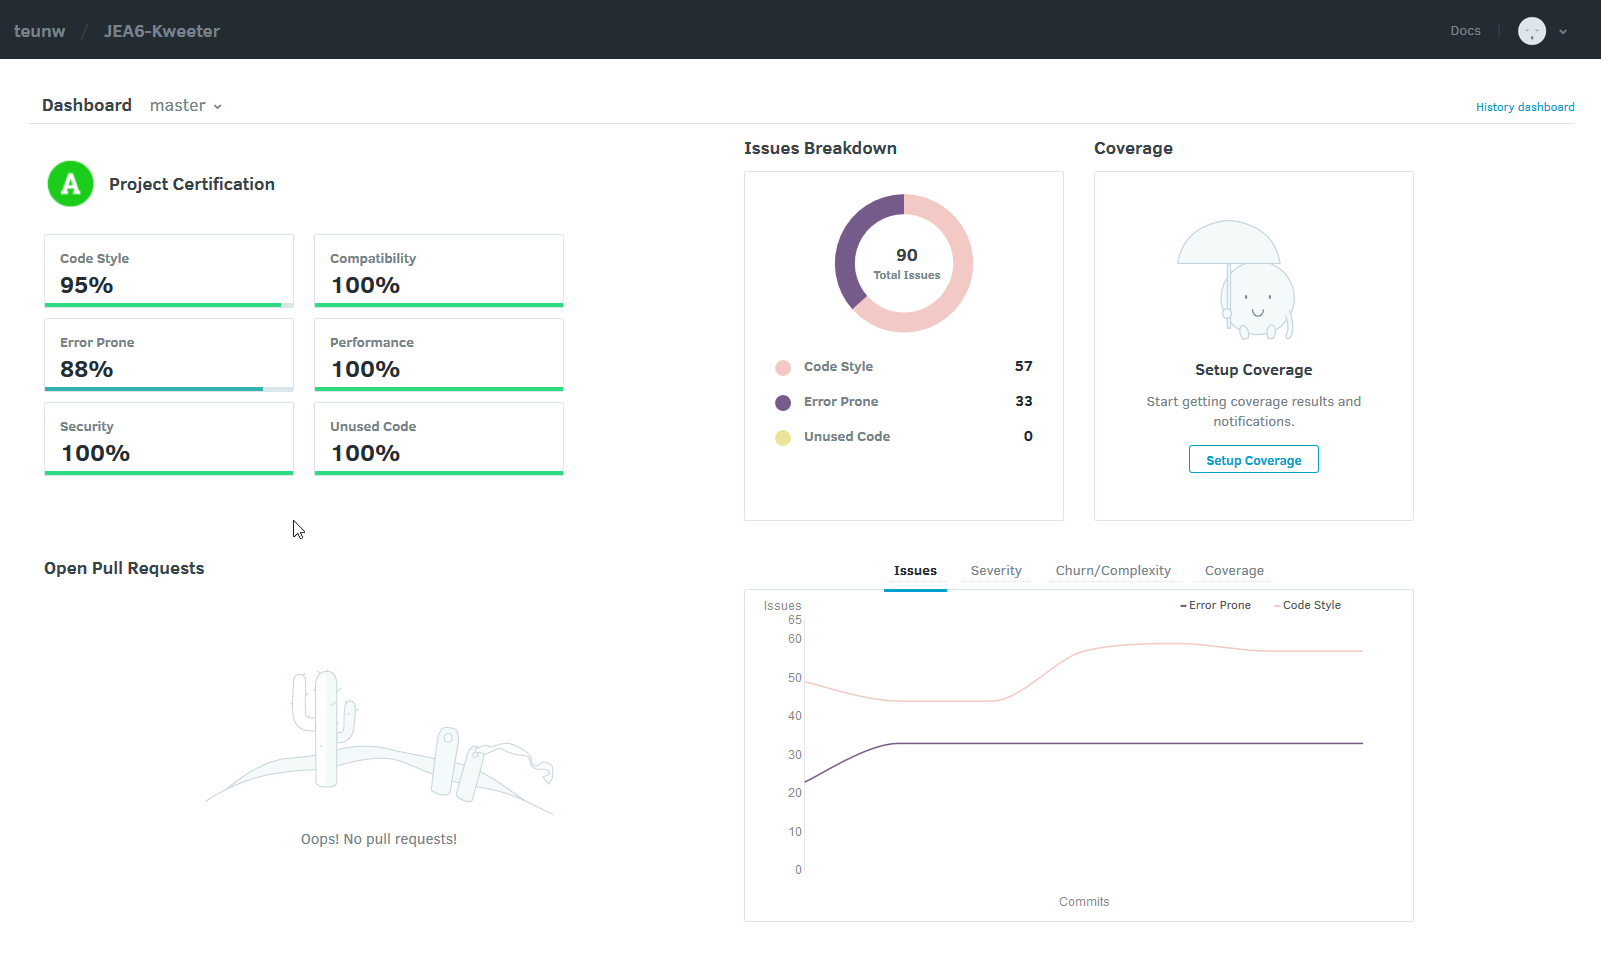
\includegraphics[width=0.75\textwidth]{images/StaticCodeAnalysis.png}
	\caption{Voorbeeld van code analysis door middel van Codacy}
	\label{fig:StaticCodeAnalyses}
\end{figure}

Ook kan er gecontroleerd worden op beveiligingsproblemen in je applicatie, stel dat je bijvoorbeeld SQL-query parameters in je queries hebt staan, dan wordt dat netjes gerapporteerd.
Andere dingen waartegen je beschermt wordt zijn:
\begin{itemize}
	\setlength\itemsep{0em}
	\item Authentication
	\item CSRF aanvallen
	\item File access
	\item SQL Injection
	\item XSS
\end{itemize}

Natuurlijk bied Codacy ook een gedetaileerd overzicht van de verschillende fouten in je code.
\begin{figure}[H]
	\centering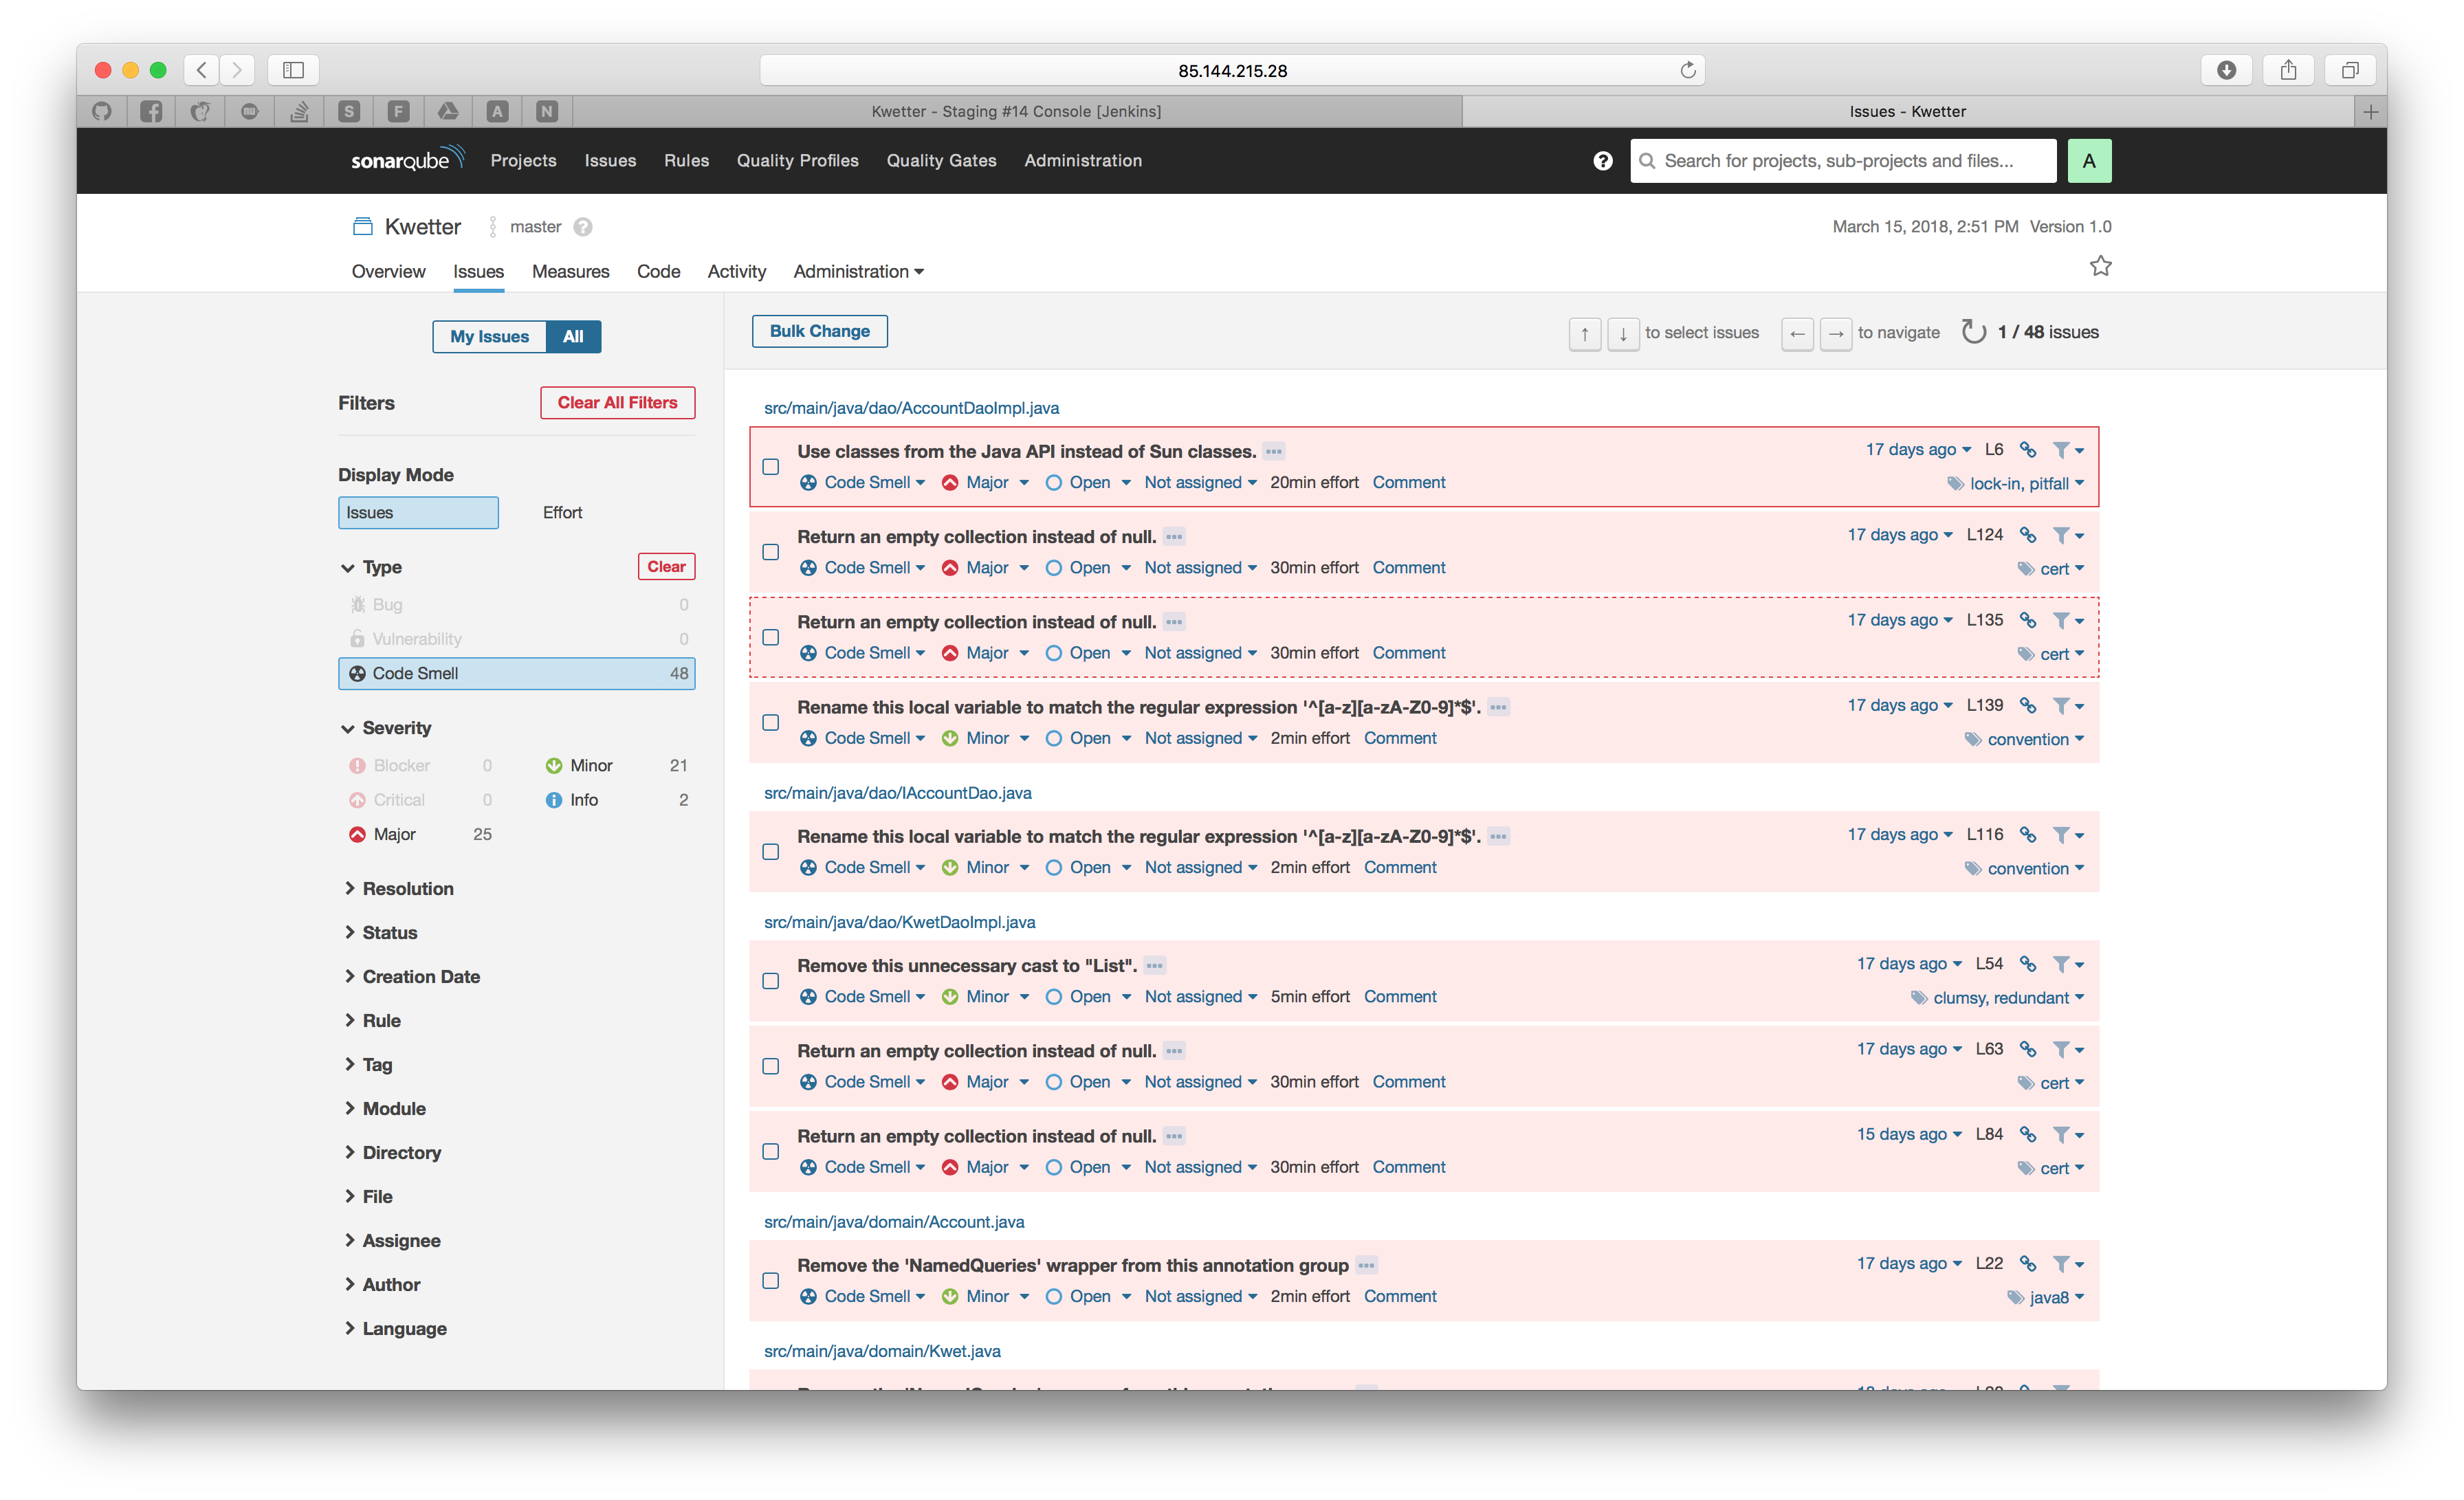
\includegraphics[width=0.5\textwidth]{images/Codacy}
	\caption{Verschillende fouten in een Typescript bestand}
\end{figure}

\section{Release}
Codacy heeft de mogelijkheid om branches individueel te controleren op code.
Hierdoor kan je per branch inzien wat voor cijfer deze krijgen.
Branches worden aan een hoge standaard gehouden, de code moet minimaal een A krijgen om te mogen mergen met de development.
\begin{figure}[H]
	\centering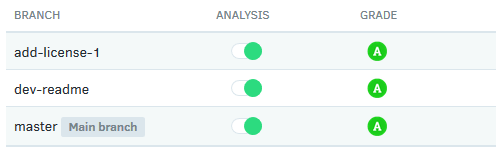
\includegraphics[width=0.55\textwidth]{images/CodacyBranchGrades}
	\caption{Branches en hun cijfer}
\end{figure}
Er is geen infrastructuur om te zorgen dat code met een laag cijfer niet gemerged kan worden, dit is een limitatie van de infrastructuur (dus van Github en Codacy).
Op hotfix branches hoeft niet meteen een controle uitgevoerd te worden, aangezien een hotfix zo snel mogelijk live moet zijn is dit onwenselijk.
Wel zou deze controle uitgevoerd moeten worden nadat de hotfix toegepast is, omdat slechte code in deze branch het mergen van andere zou kunnen hinderen.
De ontwikkelaar is verantwoordelijk voor zijn/haar eigen branch, het is de taak van de ontwikkelaar om een slecht cijfer te repareren.
